\begin{frame}
\frametitle{Example Images}
Some example (non-brain) images.
\begin{center}
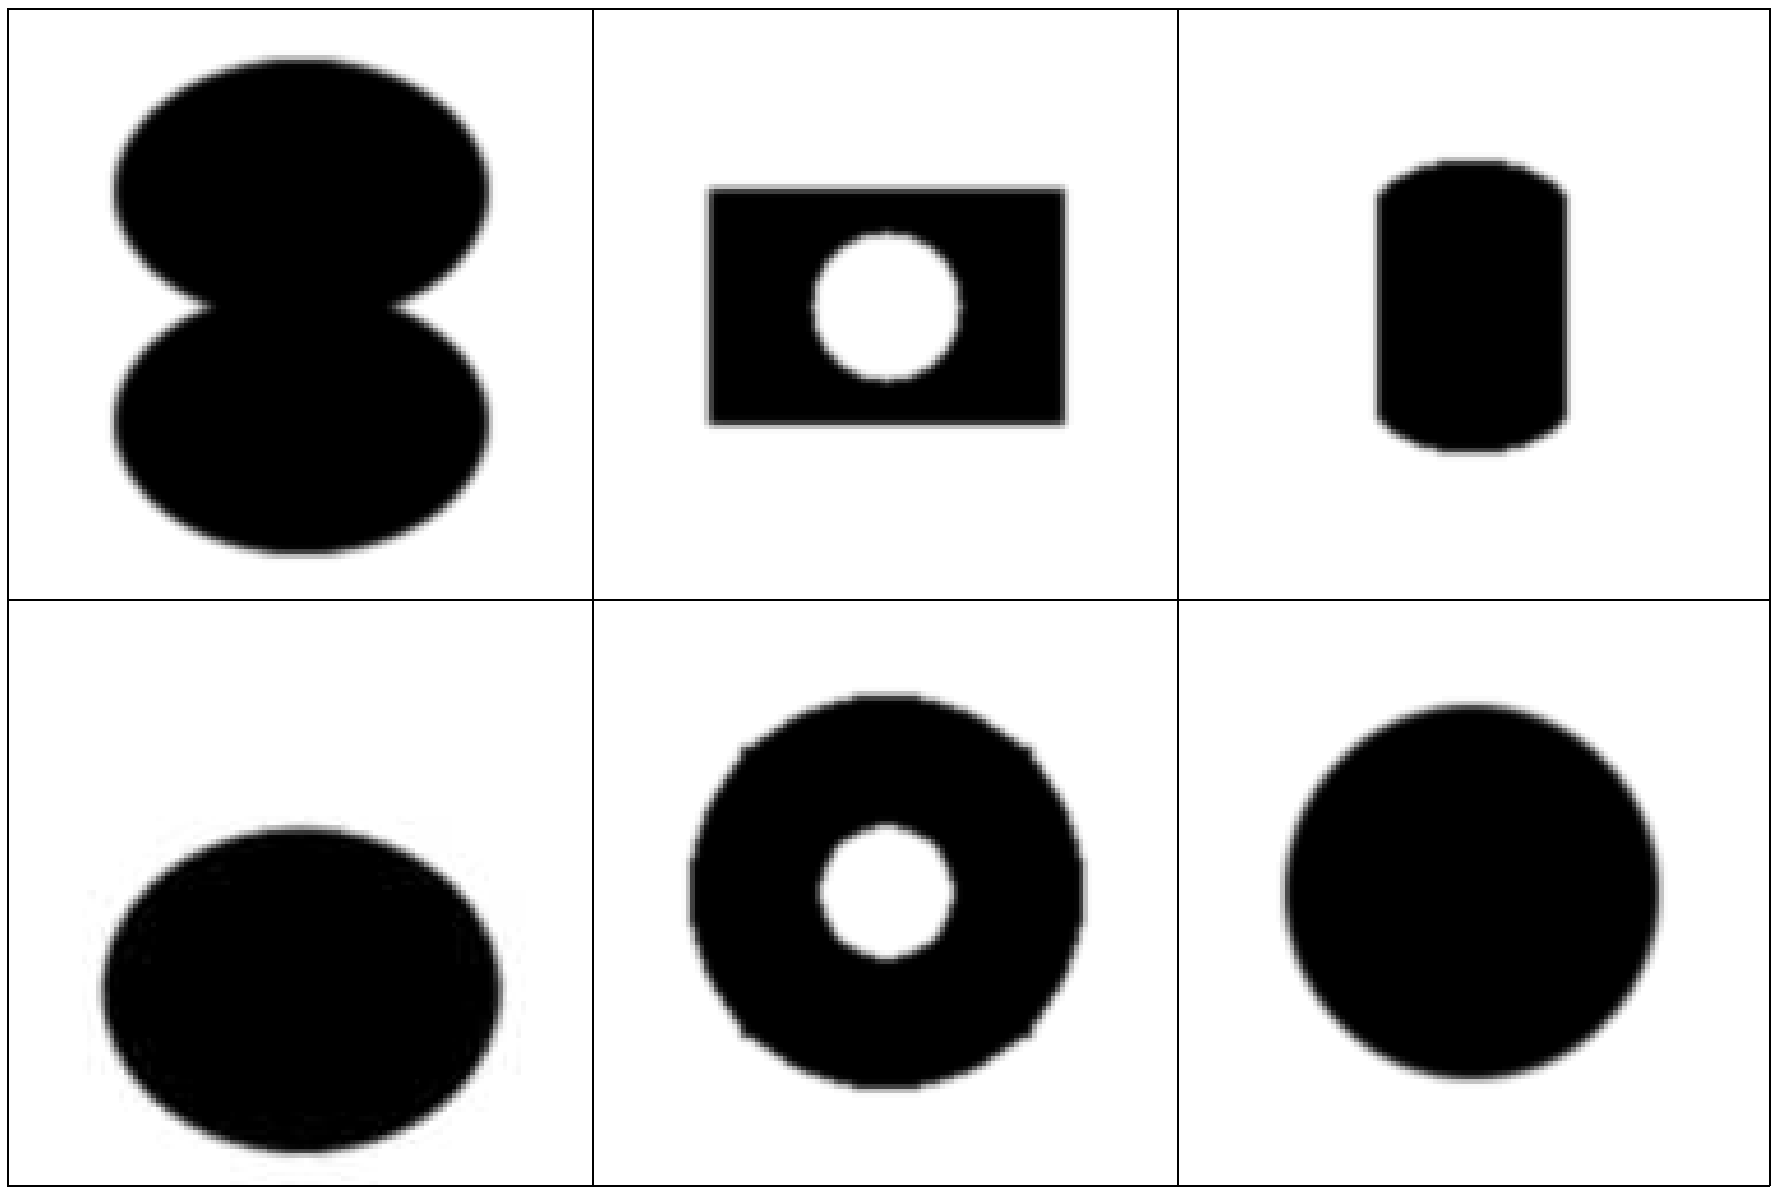
\includegraphics[width=0.9\textwidth]{original}
\end{center}
\end{frame}

%\begin{frame}
%\frametitle{Samples from a Linear Generative Model}
%Did the images come from a model like this?
%\begin{center}
%\includegraphics[width=0.9\textwidth]{simulated_lin}
%\end{center}
%\end{frame}

%\begin{frame}
%\frametitle{Samples from a Geometric Generative Model}
%Or one like this?
%\begin{center}
%\includegraphics[width=0.9\textwidth]{simulated}
%\end{center}
%\end{frame}

\begin{frame}
\frametitle{Registered Images}
We could register the images to their average shape...
\begin{center}
\includegraphics[width=0.9\textwidth]{warped}
\end{center}
\end{frame}

\begin{frame}
\frametitle{Deformations}
...and study the deformations...
\begin{center}
\includegraphics[width=0.9\textwidth]{deformations}
\end{center}
\end{frame}

\begin{frame}
\frametitle{Jacobian Determinants}
...or the relative volumes...
\begin{center}
\includegraphics[width=0.9\textwidth]{jacobians}
\end{center}
\end{frame}

\begin{frame}
\frametitle{Scalar Momentum}
... or ``scalar momentum'' (Singh et al, MICCAI 2010).
\begin{center}
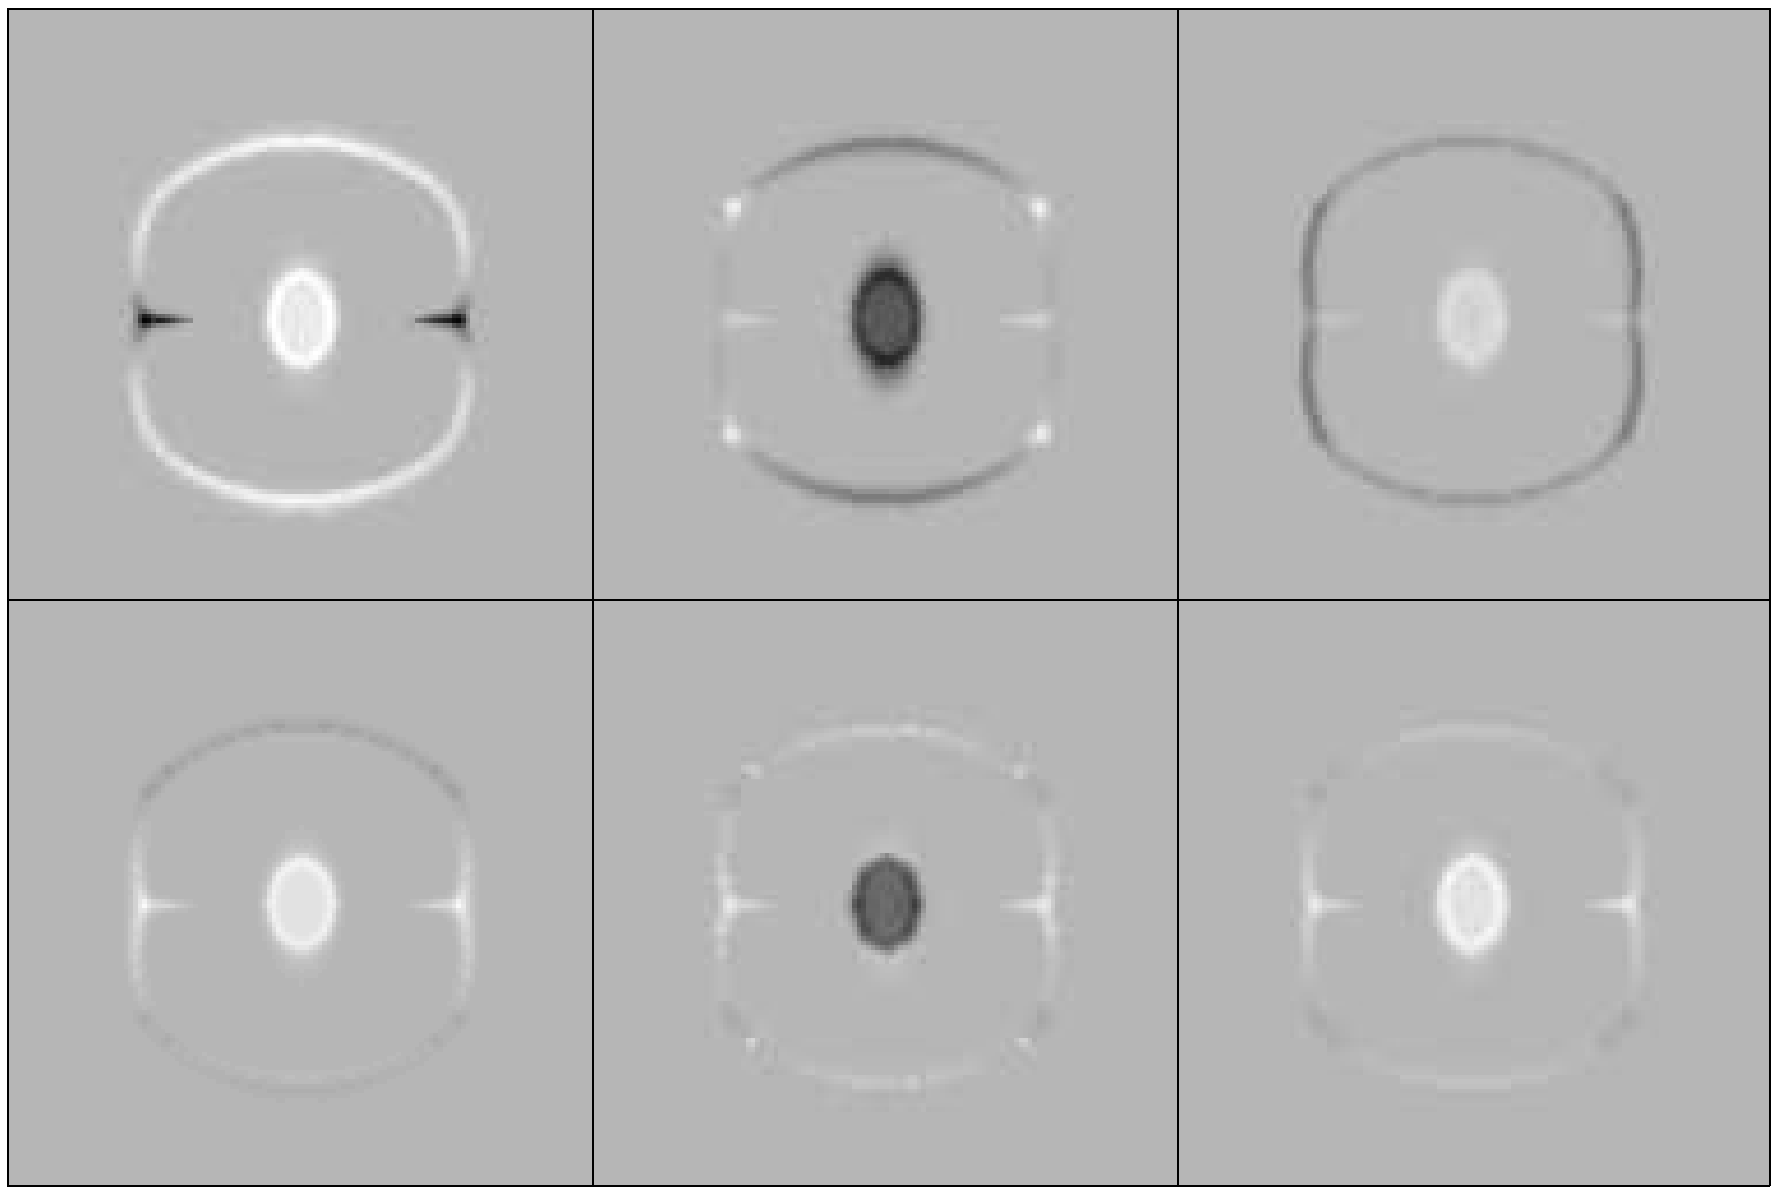
\includegraphics[width=0.9\textwidth]{alpha}
\end{center}
\end{frame}

\begin{frame}
\frametitle{Reconstructed Images}
Reconstructions from template and scalar momenta.
\begin{center}
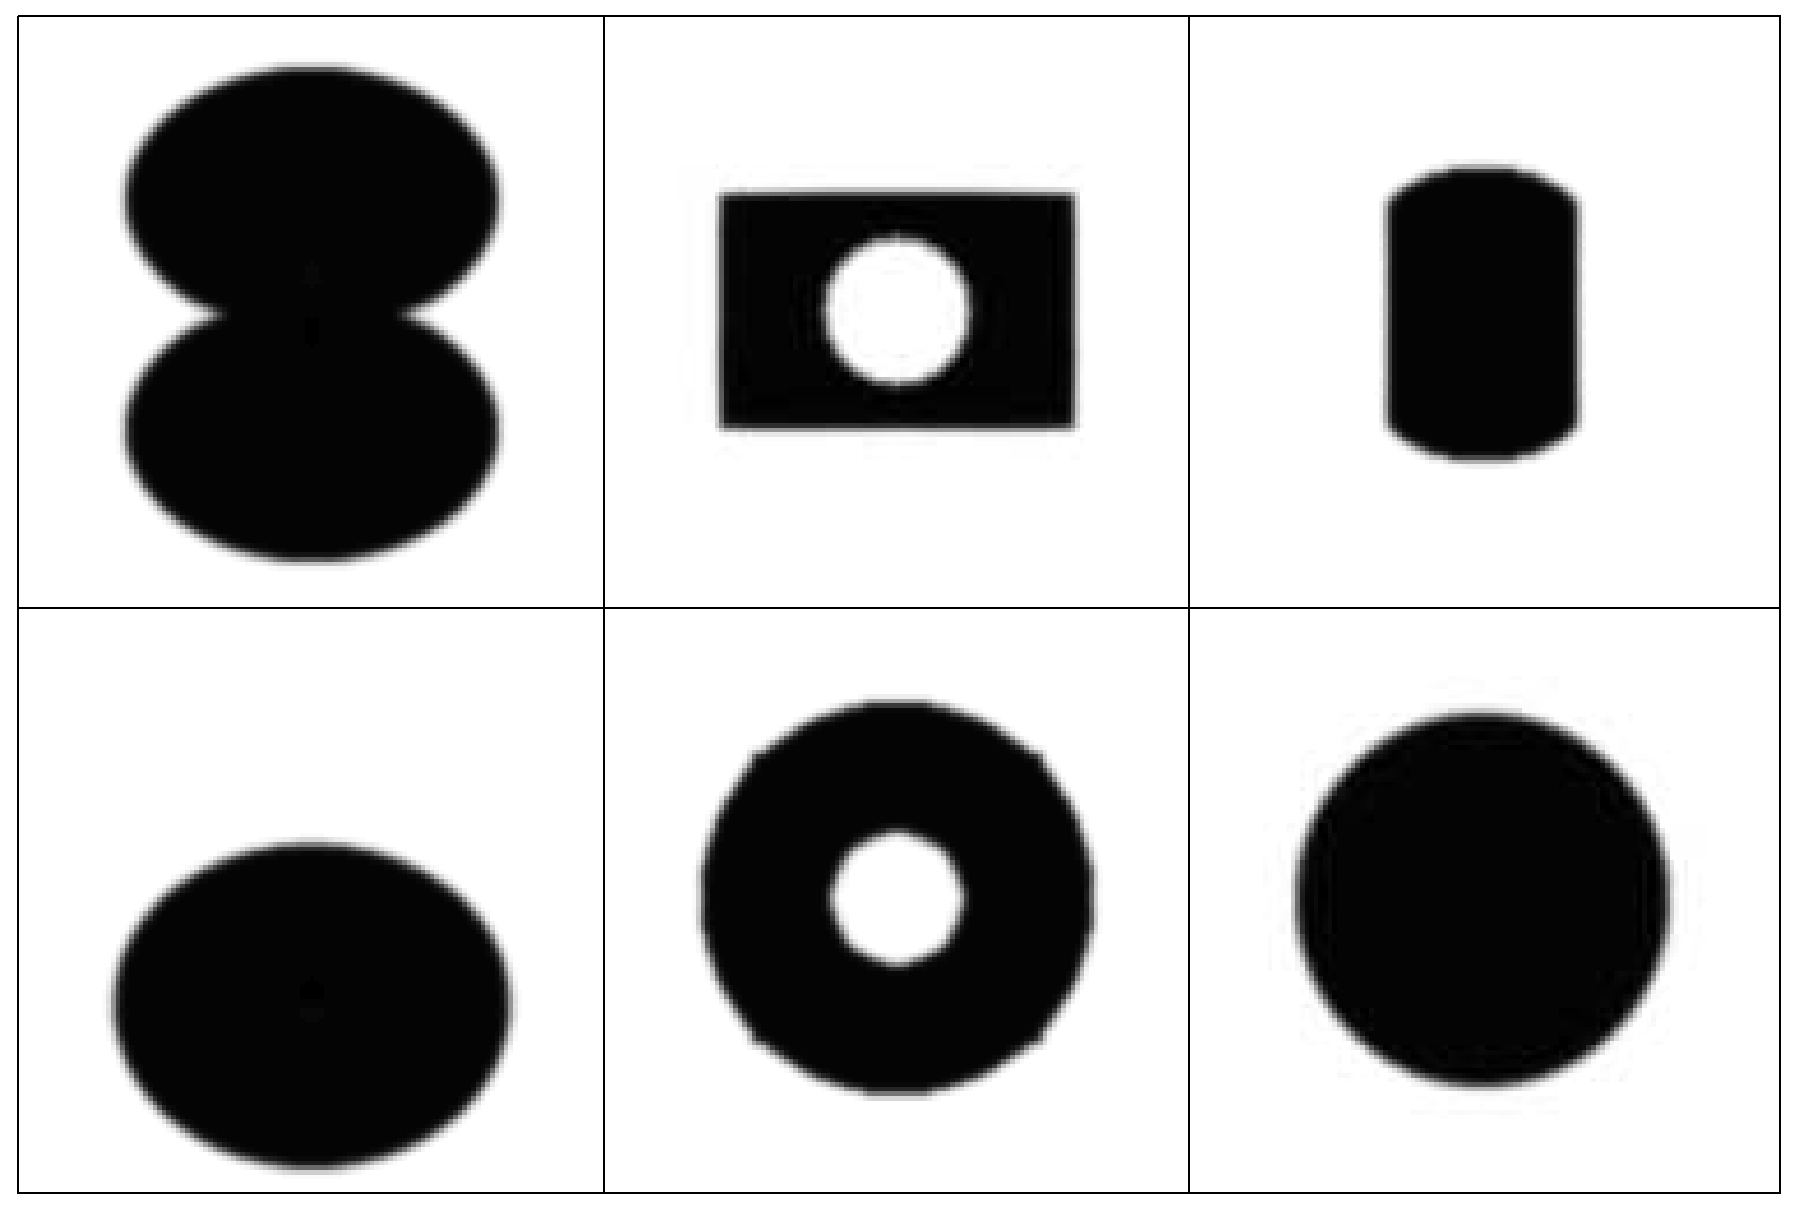
\includegraphics[width=0.9\textwidth]{reconstructed}
\end{center}
\end{frame}

%\begin{frame}
%\frametitle{Evolution}
%\begin{center}
%\includegraphics[width=.8\textwidth]{evolution}\par
%\begin{tiny}
%Singh, Fletcher, Preston, Ha, King, Marron, Wiener \& Joshi (2010). \emph{Multivariate Statistical Analysis of Deformation Momenta Relating Anatomical Shape to Neuropsychological Measures}. T. Jiang et al. (Eds.): MICCAI 2010, Part III, LNCS 6363, pp. 529--537, 2010.\par
%\end{tiny}
%\end{center}
%\end{frame}

